%
% teil2.tex -- Beispiel-File für teil2 
%
% (c) 2020 Prof Dr Andreas Müller, Hochschule Rapperswil
%
% !TEX root = ../../buch.tex
% !TEX encoding = UTF-8
%
\section{Zusammenhang mit Möbius Transformation
\label{geradlinig:section:zusammenhang_mit_moebius_transformation}}
\kopfrechts{Zusammenhang mit Möbius Transformation}
Die Möbius-Transformation ist eine Abbildung auf der komplexen Zahlenebene der Form
\begin{align*}
    f(z)=\frac{az+b}{cz+d},
\end{align*}
wobei $a,b,c,d\in\mathbb{C}$ und $ad-bc\neq0$ gilt.
Möbius-Transformationen werden in Kapitel~\ref{chapter:moebius}
ausführlicher behandelt.
In diesem Abschnitt beschränken wir uns auf den Elementartyp
\begin{align}
    f(z)=\frac{1}{z}
    \label{eq:mt_inv}
\end{align}
der Möbius-Transformation.
Dieser Elementartyp wird ebenfalls als Inversion bezeichnet.
Er ist jedoch nicht mit der geometrischen Kreisspiegelung 
auf der komplexen Zahlenebene identisch, 
auch wenn beide Abbildungen ähnliche Eigenschaften besitzen.
In diesem Paper wird die Bezeichnung Inversion 
weiterhin ausschliesslich für die Kreisspiegelung verwendet.

\subsection{Inversion}
Die Kreisspiegelung wird in der komplexen Zahlenebene durch
\begin{align}
    f(z)=\frac{R^2}{\overline{z}}
    \label{eq:inversion}
\end{align}
beschrieben, wobei $z\in\mathbb{C}$ und $\overline{z}$ 
die komplexe Konjugation von $z$ bezeichnet.
Sie entspricht der geometrischen Kreisspiegelung 
an einem Kreis mit Mittelpunkt im Ursprung und Radius $R$.

Der wesentliche Unterschied zum Elementartyp aus~\eqref{eq:mt_inv} 
besteht in der komplexen Konjugation.
Dadurch kehrt die Kreisspiegelung die Orientierung um und 
ist nicht holomorph.
Die Abbildung~\eqref{eq:inversion} ist dagegen holomorph für
$z\neq0$ und erhält die Orientierung.
Damit können wir die Gleichung~\eqref{eq:constant0}
der Kreisspiegelung folgendermassen erweitern:
\begin{align*}
    \overline{MP} \cdot \overline{MP'} 
    = 
    |z| \cdot |f(z)|
    = 
    |z| \cdot \frac{R^2}{|\overline{z}|} 
    =
    |z| \cdot \frac{R^2}{|z|} 
    = R^2.
\end{align*}

Abbildung~\ref{fig:moebius_transform} zeigt die Wirkung der Inversion.
Kreise werden wieder auf Kreise abgebildet.
Geraden bilden dabei den Grenzfall eines Kreises mit 
unendlichem Radius.
Deshalb können auch Geraden auf Kreise und Kreise auf 
Geraden abgebildet werden.
Diese Eigenschaft wird als Kreistreue bezeichnet.
Sie besagt, dass Kreise und Geraden unter einer Möbius-Transformation 
stets wieder auf Kreise oder Geraden abgebildet werden.
Zusätzlich ist die Inversion winkeltreu.
Das bedeutet, dass sich die Schnittwinkel zweier Kurven unter 
der Abbildung nicht ändern.
In Abbildung~\ref{fig:moebius_transform} bleibt der rechte Winkel 
zwischen den Kreisen daher erhalten.
\begin{figure}
    \centering
    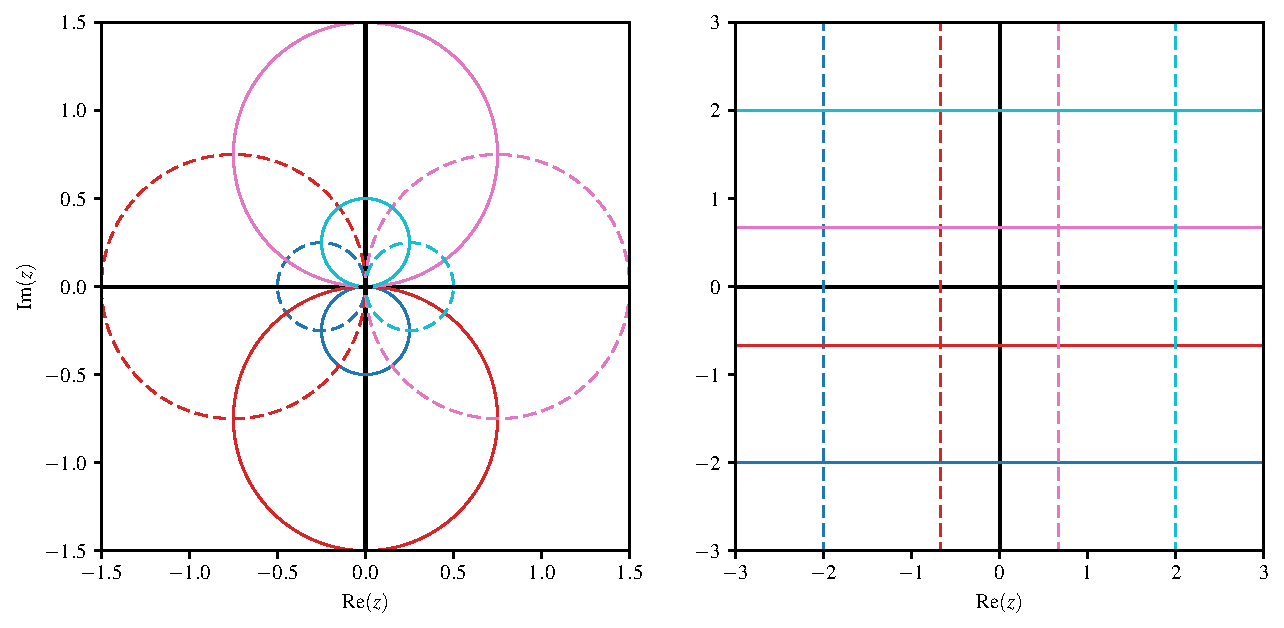
\includegraphics[width=\textwidth]{papers/geradlinig/figures/moebius_transform_plot.pdf}
    \caption{Inversion auf der komplexen Zahlenebene. 
    Kreise werden in Gerade abgebildet.}
    \label{fig:moebius_transform}
\end{figure}

Um zu zeigen, dass die geometrische Kreisspiegelung und die komplexe 
Inversion gemäss~\eqref{eq:inversion} 
dieselbe Abbildung beschreiben, 
betrachten wir Abbildung~\ref{fig:compl_inv}.
Dort sind rote Kreise dargestellt, 
welche mithilfe der komplexen Inversion transformiert werden.
Zusätzlich ist der grüne Inversionskreis eingezeichnet, 
der aus der geometrischen Kreisspiegelung bekannt ist.
Man erkennt, dass sich Kreise, 
welche sich dem Inversionskreis annähern, 
im Bild zunehmend wie Geraden verhalten.
Dies stimmt mit der Eigenschaft der geometrischen Kreisspiegelung 
aus Gleichung~\eqref{eq:constant0} überein.
Befindet sich ein Punkt auf dem Inversionskreis, 
so wird er auf sich selbst abgebildet.
Verläuft ein Kreis durch den Ursprung beziehungsweise 
durch den Mittelpunkt des Inversionskreises, 
so wird er auf eine Gerade abgebildet.
Verläuft ein Kreis hingegen nicht durch den Ursprung, 
wie in Abbildung~\ref{fig:compl_inv} in der linken Hälfte dargestellt, 
so bleibt sein Bild wiederum ein Kreis.
\begin{figure}
    \centering
    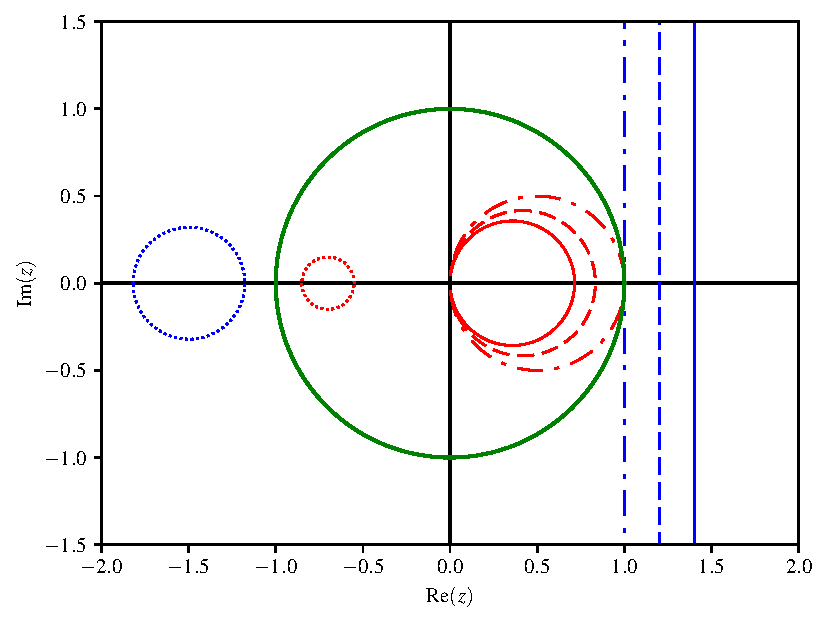
\includegraphics[width=0.6\textwidth]{papers/geradlinig/figures/inversion_plot.pdf}
    \caption{Komplexe Inversion mit eingezeichnetem Inversionskreis. 
    Kreise, die durch den Ursprung verlaufen, 
    werden auf Geraden abgebildet.}
    \label{fig:compl_inv}
\end{figure}

Die vorgestellten Mechanismen zur Erzeugung geradliniger 
Bewegungen setzen 
die Eigenschaften der komplexen Inversion beziehungsweise
eines Elementartyps der Möbius-Transformation auf rein mechanische 
Weise um.
Für ihre Entwicklung wurde jedoch nicht die Theorie 
der Möbius-Transformationen verwendet, sondern 
die geometrische Kreisspiegelung.
Diese beschreibt dieselben grundlegenden Zusammenhänge 
in einer anschaulicheren geometrischen Form.
Dennoch genügt die Kreisspiegelung allein nicht zur Entwicklung 
solcher Mechanismen.
Ihre Konstruktion erforderte zusätzlich Kreativität, 
Erfindergeist und zahlreiche experimentelle Untersuchungen.
Unabhängig von ihrer historischen Entstehung spiegeln 
diese Mechanismen die mathematischen Eigenschaften 
der komplexen Inversion auf bemerkenswerte Weise wider.